Взятая за основу схема БПЛА-ЦАГИ выполнена по схеме ``бесхвостка''. Габаритные размеры БПЛА: 
\begin{itemize}
\item размах крыльев: $\approx37\text{м}$
\item высота фюзеляжа: 1.7м
\item длина фюзеляжа: 7м
\end{itemize}


Пока кратко: Крыло большого удлинения интегрировано с фюзеляжем. Двигатель утоплен в конструкцию, подвод воздухозаборника, сопло над горизонтальным оперением. В передней части фюзеляжа расположены отсеки с БРЭО, отсеки с топливом, отсек под переднее шасси. 
В задней части фюзеляжа пара отсеков под топливо, отсеки под БРЭО, шассийные отсеки, шасси крепится на стыке крыла с фюзеляжем. 

\begin{figure}
\caption{Модель БПЛА-ЦАГИ, вид сверху}
\label{fig:BPS_topview}
\end{figure}



\begin{figure}[H]
\centering
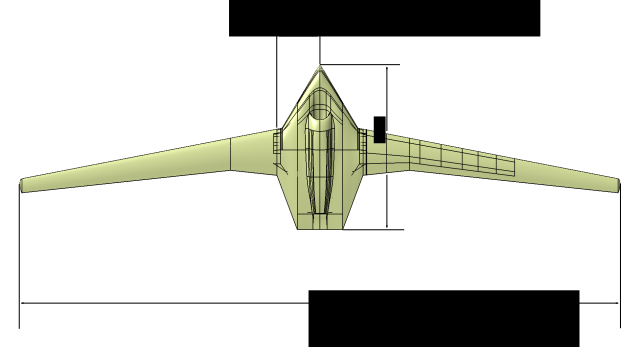
\includegraphics[width=0.8\textwidth]{BPS_Catia_Top}
\caption{Вид сверху}
\label{fig:BPS_Catia_Top}
\end{figure}

\begin{figure}[H]
\centering
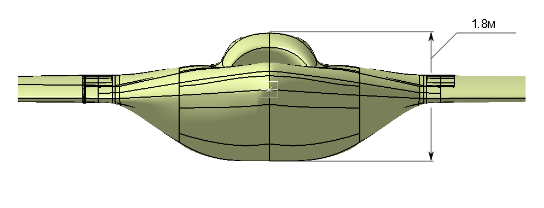
\includegraphics[width=0.8\textwidth]{BPS_Catia_Front}
\caption{Вид фюзеляжа спереди}
\label{fig:BPS_Catia_Front}
\end{figure}

\begin{figure}[H]
\centering
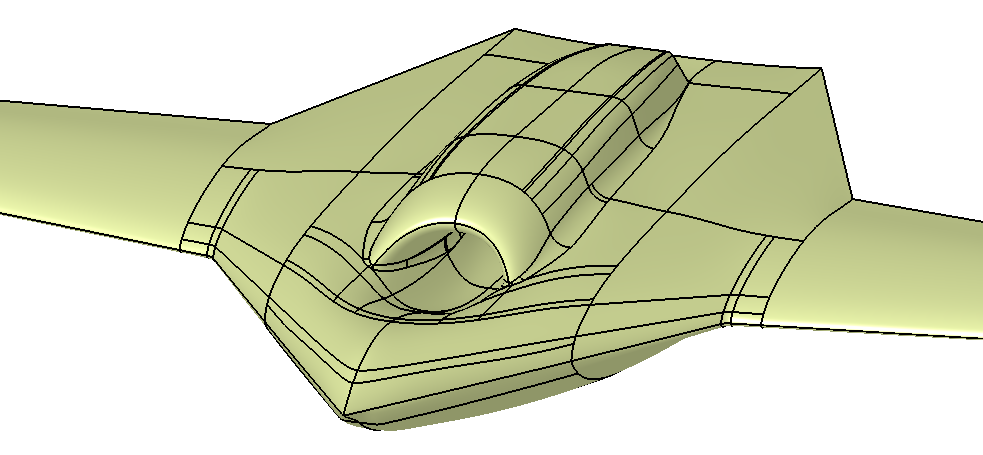
\includegraphics[width=0.8\textwidth]{BPS_Catia}
\caption{Вид фюзеляжа в изометрии}
\label{fig:BPS_Catia}
\end{figure}

\begin{figure}[H]
\centering
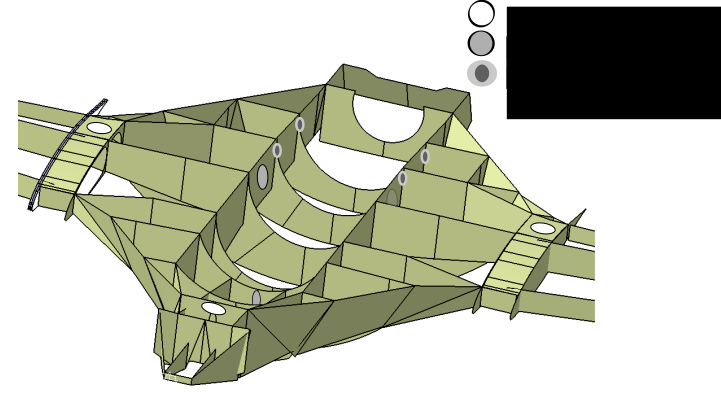
\includegraphics[width=0.8\textwidth]{BPS_Catia_WithoutSkin}
\caption{Вид фюзеляжа со снятой обшивкой}
\label{fig:BPS_Catia_WithoutSkin}
\end{figure}


%Описываем полностью всю конструкцию. Показываем много разных картинок. 